%%%%%% NORMAL BED - LEFT %%%%%%
\subsubsection{Result Normal Bed in Left Side Position}   

The estimated respiratory rate per minute (rpm) while the participants are on the left side with the mattress placed on a normal bed is further presented. Table \ref{tab:LeftNormalStillsg} presented the estimated rpm using binary and weighted approach compared with the rpm given by the ground truth. The approaches retrieve an almost identical rpm, this result may be due to the choice of the minimum confidence value at 80\% that allows keeping only the best signal, maybe with higher confidence can be seen a higher difference between the two approaches. 

\vspace{1.3cm}
%\begin{table}\begin{tabular}{|llllll|}
\hline 
Binary SGf & binary Waveleft & weighed  SGf & weighed Waveleft & resp rate & toolbox \\ 
\hline 
13.375 & 14.6364 & 13.375 & 14.6364 & 11.2045 & 10 \\ 
13.6667 & 15 & 13.6667 & 15 & 12.7397 & 11 \\ 
14 & 16 & 13.5 & 15.25 & 13.0613 & 12 \\ 
14.3571 & 14.2 & 14.3571 & 14.2 & 12.2669 & 12 \\ 
14 & 19 & 14 & 19 & 12.1628 & 13 \\ 
12.8 & 15 & 12.6667 & 14.5 & 13.6039 & 13 \\ 
11.8 & 14.2222 & 11.8 & 14.2222 & 13.1398 & 13 \\ 
14 & 15.6667 & 14 & 15.6667 & 11.5445 & 14 \\ 
13.8333 & 14.7 & 13.8333 & 14.7 & 10.77 & 11 \\ 
13.8889 & 15.8571 & 13.8889 & 15.8571 & 14.2216 & 12 \\ 
13.0833 & 15.5556 & 13.0833 & 15.5556 & 13.1656 & 12 \\ 
14.1111 & 16.5714 & 13.7 & 16.5714 & 12.9764 & 12 \\ 
14.2 & 15 & 14.2 & 15 & 10.9055 & 13 \\ 
13.25 & 15.125 & 13.25 & 15.125 & 13.2294 & 11 \\ 
12.7692 & 15.7143 & 12.2857 & 15.5 & 12.8524 & 11 \\ 
13.9167 & 15.2 & 13.6154 & 15.2 & 11.3824 & 13 \\ 
13 & 14.6 & 13 & 14.6 & 13.5579 & 11 \\ 
13 & 15.8889 & 13 & 15.8889 & 11.6069 & 12 \\ 
\hline 
\end{tabular}
\caption{Breath per minutes for each approach, result from Noxtural and toolbox
- Left position still mattress}
\end{table}

\begin{table}[h]
    \centering
    \begin{tabular}{|c|c|c|}
 
    \hline 
    Binary & Weighed & RPM (NOXA1) \\  
\hline 
13.375    &   13.375  &    11.2045 \\ 
13.6667    &  13.6667  &    12.7397 \\ 
14       &  13.5    &  13.0613 \\ 
14.3571   &   14.3571   &   12.2669 \\ 
14        &   14  &    12.1628 \\ 
12.8     & 12.6667  &    13.6039 \\ 
11.8    &     11.8   &   13.1398 \\ 
14      &     14  &    11.5445 \\ 
13.8333 &     13.8333  &      10.77 \\ 
13.8889   &   13.8889  &    14.2216 \\ 
13.0833    &  13.0833   &   13.1656 \\ 
14.1111   &      13.7   &   12.9764 \\ 
14.2      &   14.2  &    10.9055 \\ 
13.25     &   13.25   &   13.2294 \\ 
12.7692    &  12.2857  &    12.8524 \\ 
13.9167   &   13.6154   &   11.3824 \\ 
13       &    13   &  13.5579 \\ 
13       &    13    &  11.6069 \\ 
\hline 
\end{tabular}
\caption{Estimated rpm using binary and weighted approach of the pipeline
compared with the rpm given by the ground truth
- Normal bed and left side}
\label{tab:LeftNormalStillsg}

\end{table}

\vspace{0.5cm}

Table \ref{tab:LeftNormalStillMetricssg} present the average rpm for both approaches  
and the relative mean absolute error (MAE) and mean absolute percentage error (MAPE). As just discussed in the previous paragraph there is no substantial difference between the two different approaches. The data on which to focus more is the number of breaths that the algorithm misses, represented by MAE and expressed in percentage by MAPE. The average number is 2.5rpm, which means that if we consider the estimated average of 15.3rpm the error is over 24\%, worst than in the supine position, probably due to the smaller contact area between the body and the mattress.

\vspace{1cm}
\begin{table}[H]
    \centering
    \begin{tabular}{|c|c|c|}
    \hline 
    & Binary SGf & Weighed  \\ 
    \hline 
    rpm mean &13.5029 &  13.4012\\
    MAE rpm & 1.3922 &     1.3591 \\ 
    MAPE  & 11.8278 \% & 11.5556 \% \\ 
    \hline 
    \end{tabular}
    
    \caption{Evarage number of breath for each approach with the relative mean
    absolute error (MAE) and mean absolute percentage error (MAE) - Normal bed
    and left side}
    \label{tab:LeftNormalStillMetricssg}    
\end{table}
    
    
\vspace{0.5cm}

Figure \ref{fig:baln2} show the Bland–Altman plot, presented in section \ref{cap:plottino}, of the estimated rpm from the pipeline compared to the value of the ground truth. It helps to visualize the data from Table \ref{tab:LeftNormalStillMetricssg} in respect of the error. Since the result for the approaches is similar the data presented with this plot refers to the weighted approach only.

Figure \ref{fig:rec} shows the denoised signal using MODWTMRA with the highest accuracy (92\%) for the supine position with a normal mattress.

\begin{figure}[p]
  \centering
  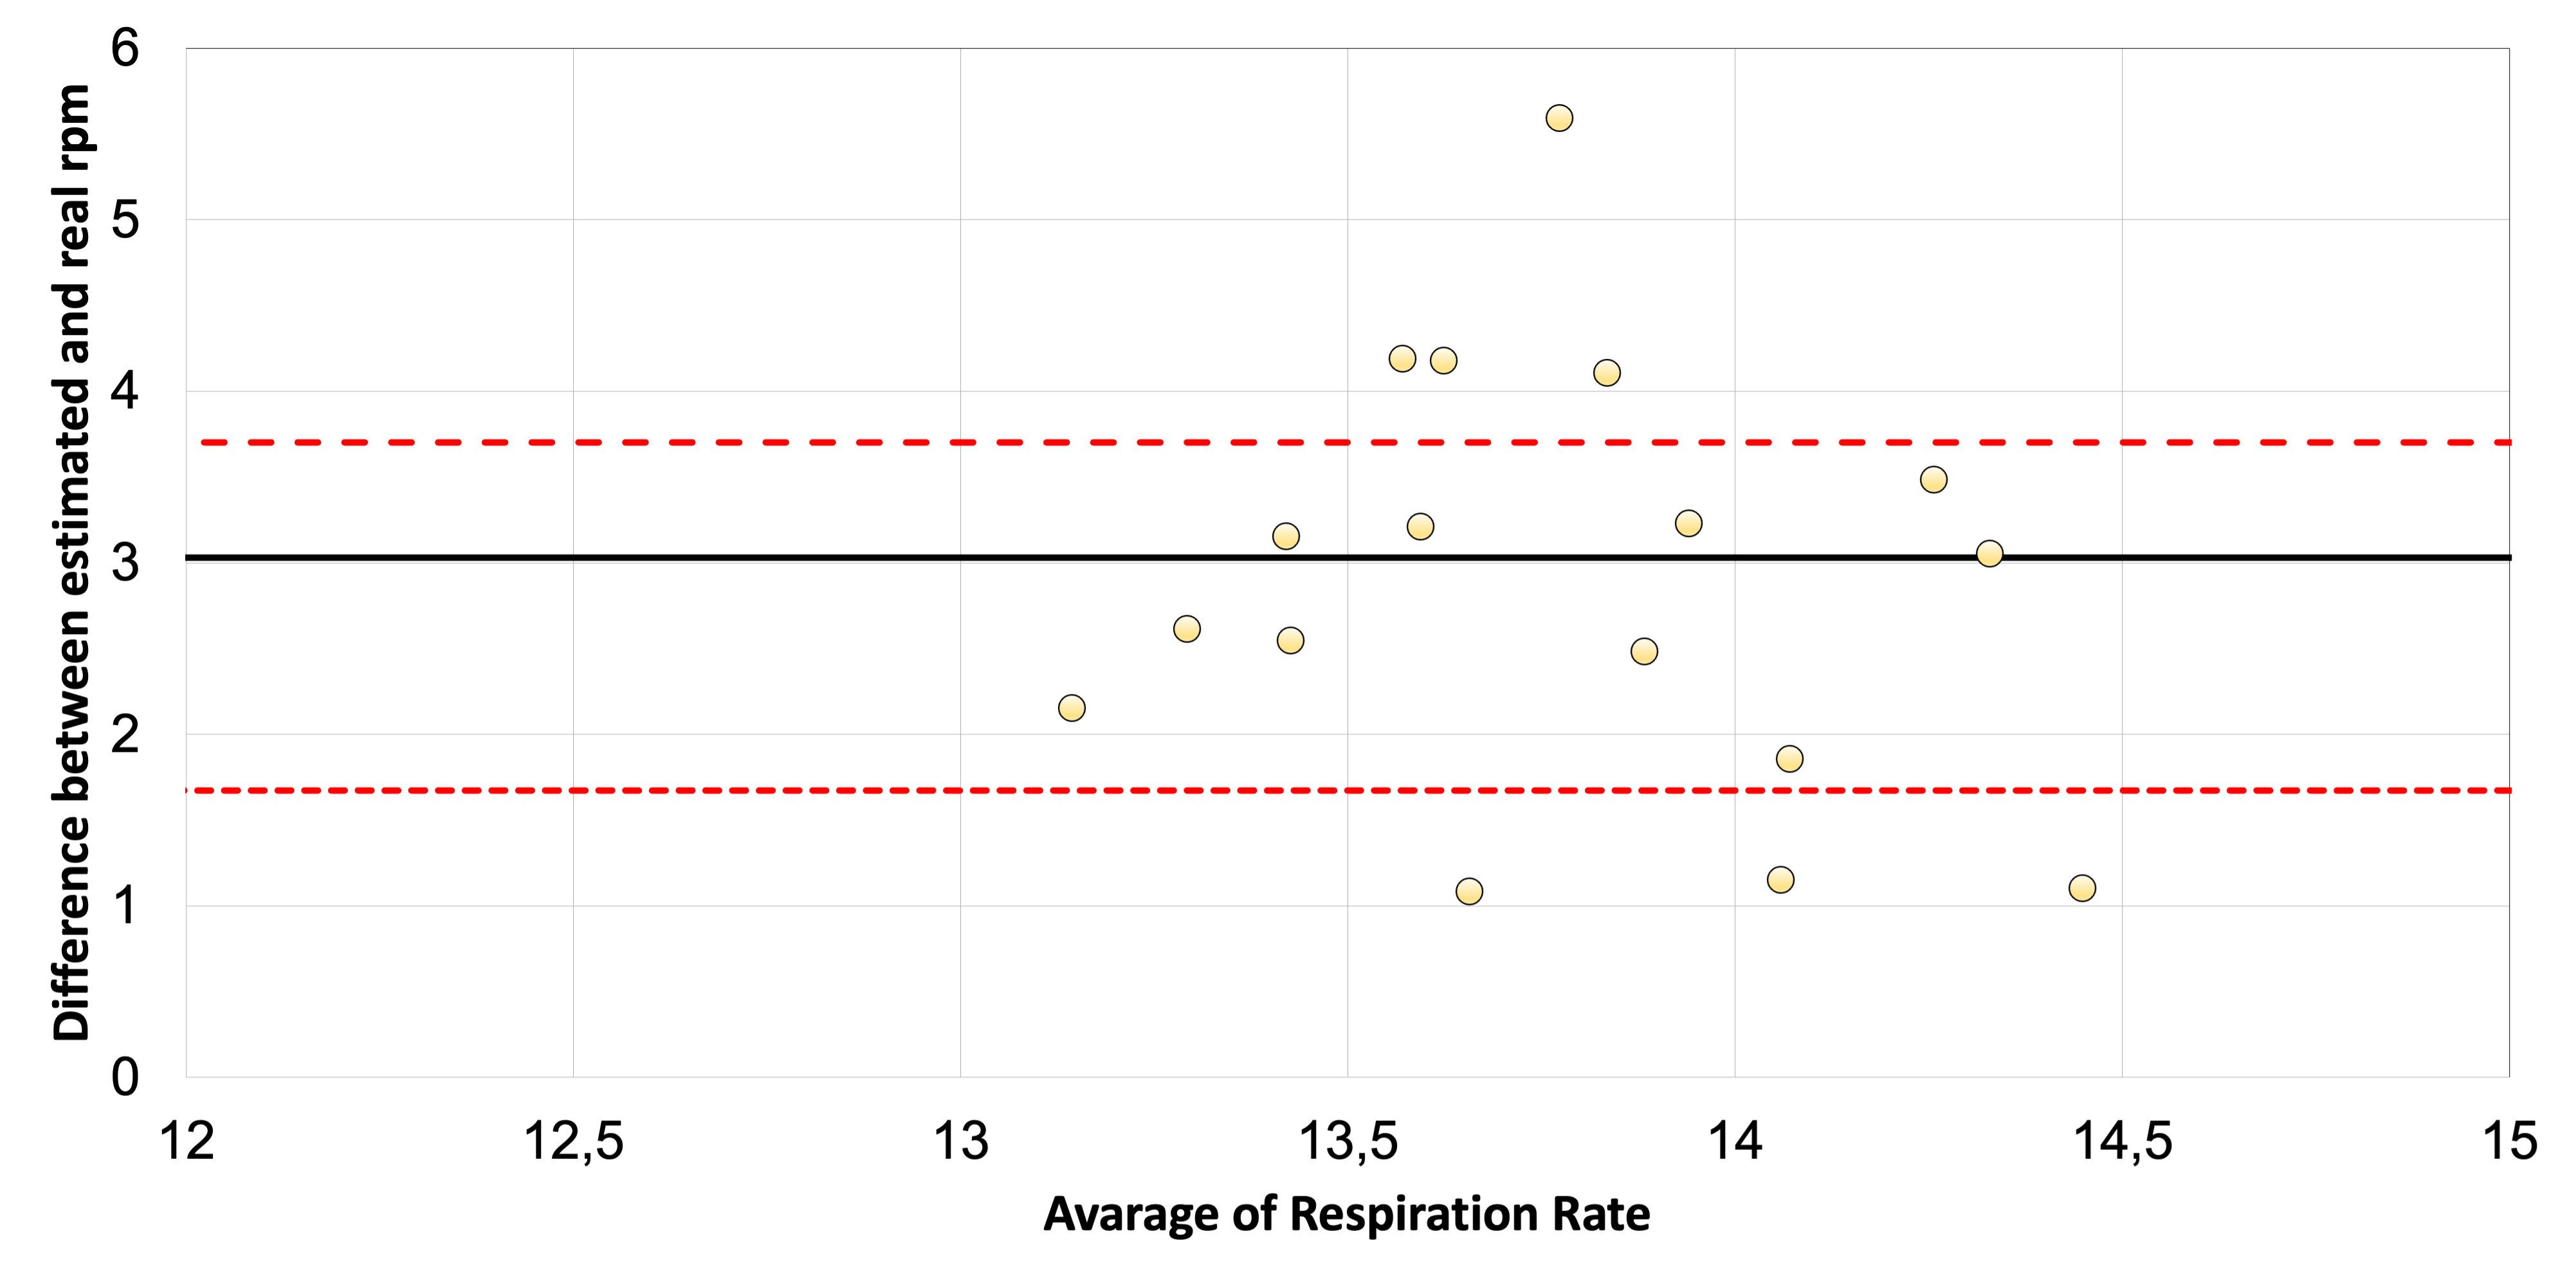
\includegraphics[width=\textwidth]{img/balnd2.png}

  \caption{Bland Altman Plot of estimated rpm from the pipeline compared to the value of the ground truth - Normal bed and left side}
  \label{fig:baln2}
  \vspace{1.5cm}
  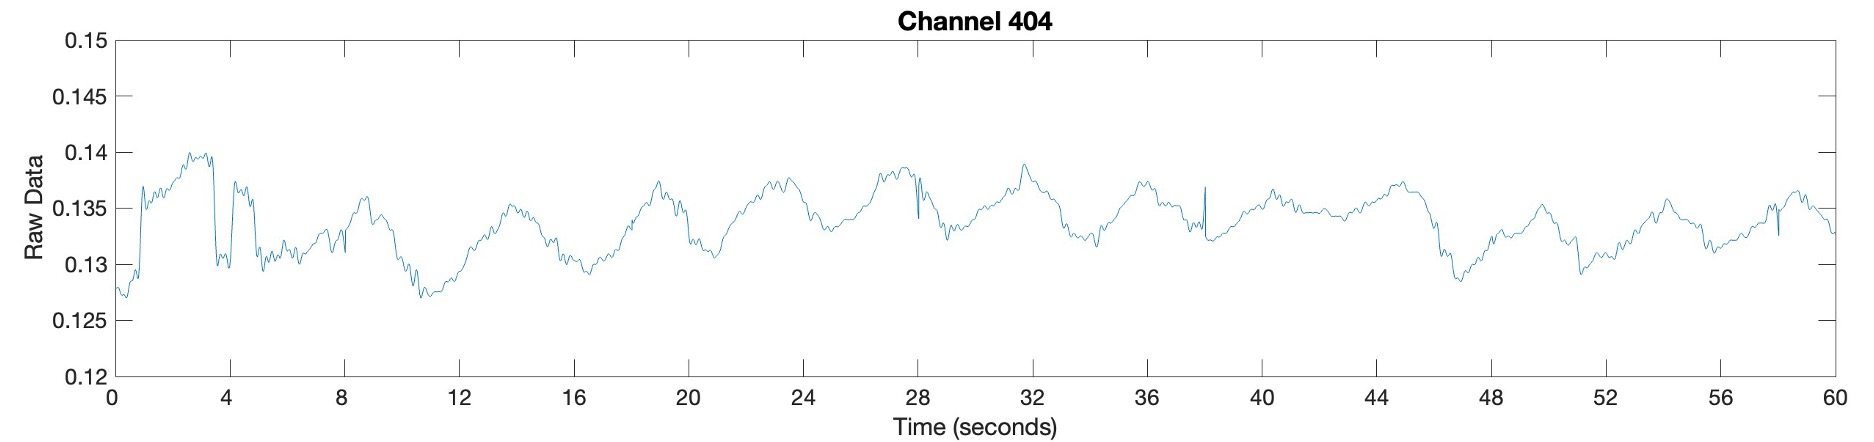
\includegraphics[width=\textwidth]{img/404.jpg}
  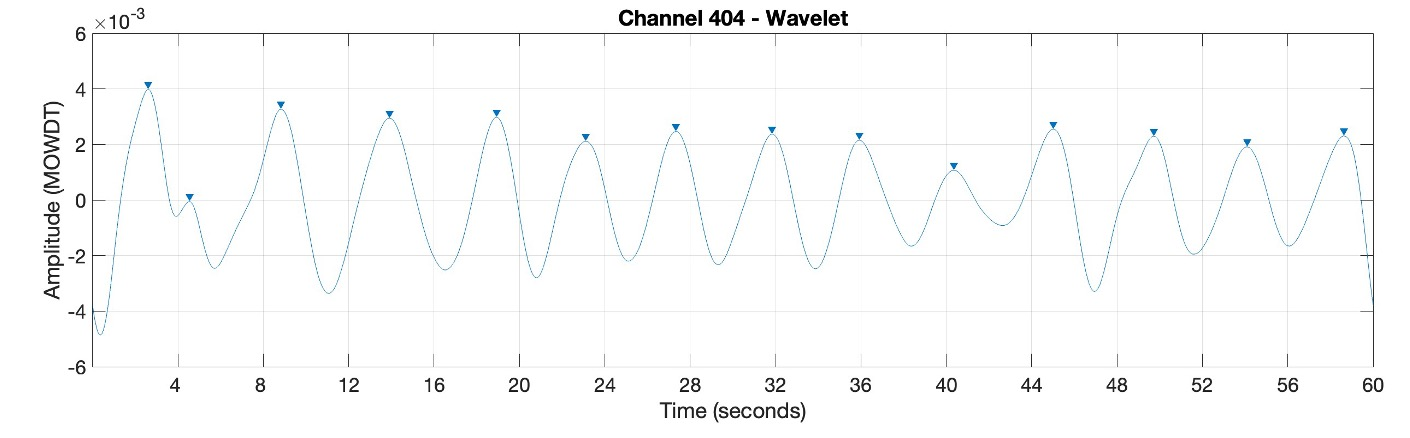
\includegraphics[width=\textwidth]{img/404_wave.jpg}
\caption{Raw data and denoised signal using MODWTMRA of the channel with the highest percentage of confidence (92\%) - Normal bed and supine position}
  \label{fig:rec}
\end{figure}


\clearpage
%%%%%% NORMAL BED - PRONE %%%%%%
\subsubsection{Result Normal Bed in Prone Side Position}   

The estimated respiratory rate per minute (rpm) while the participants are in the prone position with the mattress placed on a normal bed is further presented. Table \ref{tag:ProneNormalStillsg} presented the estimated rpm using binary and weighted approach compared with the rpm given by the ground truth. The approaches retrieve an almost identical rpm, this result may be due to the choice of the minimum confidence value at 80\% that allows keeping only the best signal, maybe with higher confidence can be seen a higher difference between the two approaches. 

\vspace{1.3cm}
%\begin{table}\begin{tabular}{|llllll|}
\hline 
Binary SGf & binary Waveleft & weighed  SGf & weighed Waveleft & resp rate & toolbox \\ 
\hline 
13.375 & 14.6364 & 13.375 & 14.6364 & 11.2045 & 10 \\ 
13.6667 & 15 & 13.6667 & 15 & 12.7397 & 11 \\ 
14 & 16 & 13.5 & 15.25 & 13.0613 & 12 \\ 
14.3571 & 14.2 & 14.3571 & 14.2 & 12.2669 & 12 \\ 
14 & 19 & 14 & 19 & 12.1628 & 13 \\ 
12.8 & 15 & 12.6667 & 14.5 & 13.6039 & 13 \\ 
11.8 & 14.2222 & 11.8 & 14.2222 & 13.1398 & 13 \\ 
14 & 15.6667 & 14 & 15.6667 & 11.5445 & 14 \\ 
13.8333 & 14.7 & 13.8333 & 14.7 & 10.77 & 11 \\ 
13.8889 & 15.8571 & 13.8889 & 15.8571 & 14.2216 & 12 \\ 
13.0833 & 15.5556 & 13.0833 & 15.5556 & 13.1656 & 12 \\ 
14.1111 & 16.5714 & 13.7 & 16.5714 & 12.9764 & 12 \\ 
14.2 & 15 & 14.2 & 15 & 10.9055 & 13 \\ 
13.25 & 15.125 & 13.25 & 15.125 & 13.2294 & 11 \\ 
12.7692 & 15.7143 & 12.2857 & 15.5 & 12.8524 & 11 \\ 
13.9167 & 15.2 & 13.6154 & 15.2 & 11.3824 & 13 \\ 
13 & 14.6 & 13 & 14.6 & 13.5579 & 11 \\ 
13 & 15.8889 & 13 & 15.8889 & 11.6069 & 12 \\ 
\hline 
\end{tabular}
\caption{Breath per minutes for each approach, result from Noxtural and toolbox
- Left position still mattress}
\end{table}

\begin{table}[h]
    \centering
    \begin{tabular}{|c|c|c|}
 
    \hline 
    Binary & Weighed & RPM (NOXA1) \\  
\hline 
15.3     &    15.3  &    11.5949 \\ 
14.8125   &   14.8125  &   11.1628 \\ 
14.2      &   14.2  &    11.0005 \\ 
14.8889   &   14.8889  &    10.4762 \\ 
13.5      &   13.5  &    10.4723 \\ 
13.8571   &   13.8571   &   9.53453 \\ 
13.8571   &   13.8571  &   9.54669 \\ 
14.3    &     14.3   &   13.5758 \\ 
15      &     15   &   11.1779 \\ 
13.9     &    13.9  &    9.53453 \\ 
13.8667   &   13.8667   &   9.58413 \\ 
13.8235   &   13.8235    &  11.8196 \\ 
14.0714    &  14.0714    &  11.8153 \\ 
13        &   13   &   9.52234 \\ 
14.4828    &  14.4828   &   10.8508 \\ 
14.3793  &    14.3793  &    10.8876 \\ 
13.7     &    13.7  &    10.9705 \\ 
14.1818   &   14.1818   &    11.237 \\ 
\hline 
\end{tabular}
\caption{Estimated rpm using binary and weighted approach of the pipeline
compared with the rpm given by the ground truth
- Normal bed and prone position}
\label{tag:ProneNormalStillsg}

\end{table}

\vspace{0.5cm}

Table \ref{tab:ProneNormalStillMetricssg} present the average rpm for both approaches  
and the relative mean absolute error (MAE) and mean absolute percentage error (MAPE). As just discussed in the previous paragraph there is no substantial difference between the two different approaches. The data on which to focus more is the number of breaths that the algorithm misses, represented by MAE and expressed in percentage by MAPE. The average number is 2.8rpm, which means that if we consider the estimated average of 15rpm the error is over 36\%, worst worse than the two previous results it may depend on the movement of the chest in the prone position changes.


\vspace{1cm}
\begin{table}[H]
    \centering
    \begin{tabular}{|c|c|c|}
    \hline 
    & Binary SGf & Weighed  \\ 
    \hline
    resp mean & 14.1734  & 14.1734 \\
    MAE rpm & 3.3532  &     3.3532  \\ 
    MAPE & 31.914 \% & 31.914 \% \\ 
    \hline 
    \end{tabular}
    \caption{Evarage number of breath for each approach with the relative mean
    absolute error (MAE) and mean absolute percentage error (MAE) - Normal bed
    and prone position}
    \label{tab:ProneNormalStillMetricssg}    
\end{table}
    
\vspace{0.5cm}

Figure \ref{fig:baln2} show the Bland–Altman plot, presented in section \ref{cap:plottino}, of the estimated rpm from the pipeline compared to the value of the ground truth. It helps to visualize the data from Table \ref{tab:ProneNormalStillMetricssg} in respect of the error. Since the result for the approaches is similar the data presented with this plot refers to the weighted approach only.

Figure \ref{fig:rec} shows the denoised signal using MODWTMRA with the highest accuracy (92\%) for the supine position with a normal mattress.

\begin{figure}[p]
  \centering
  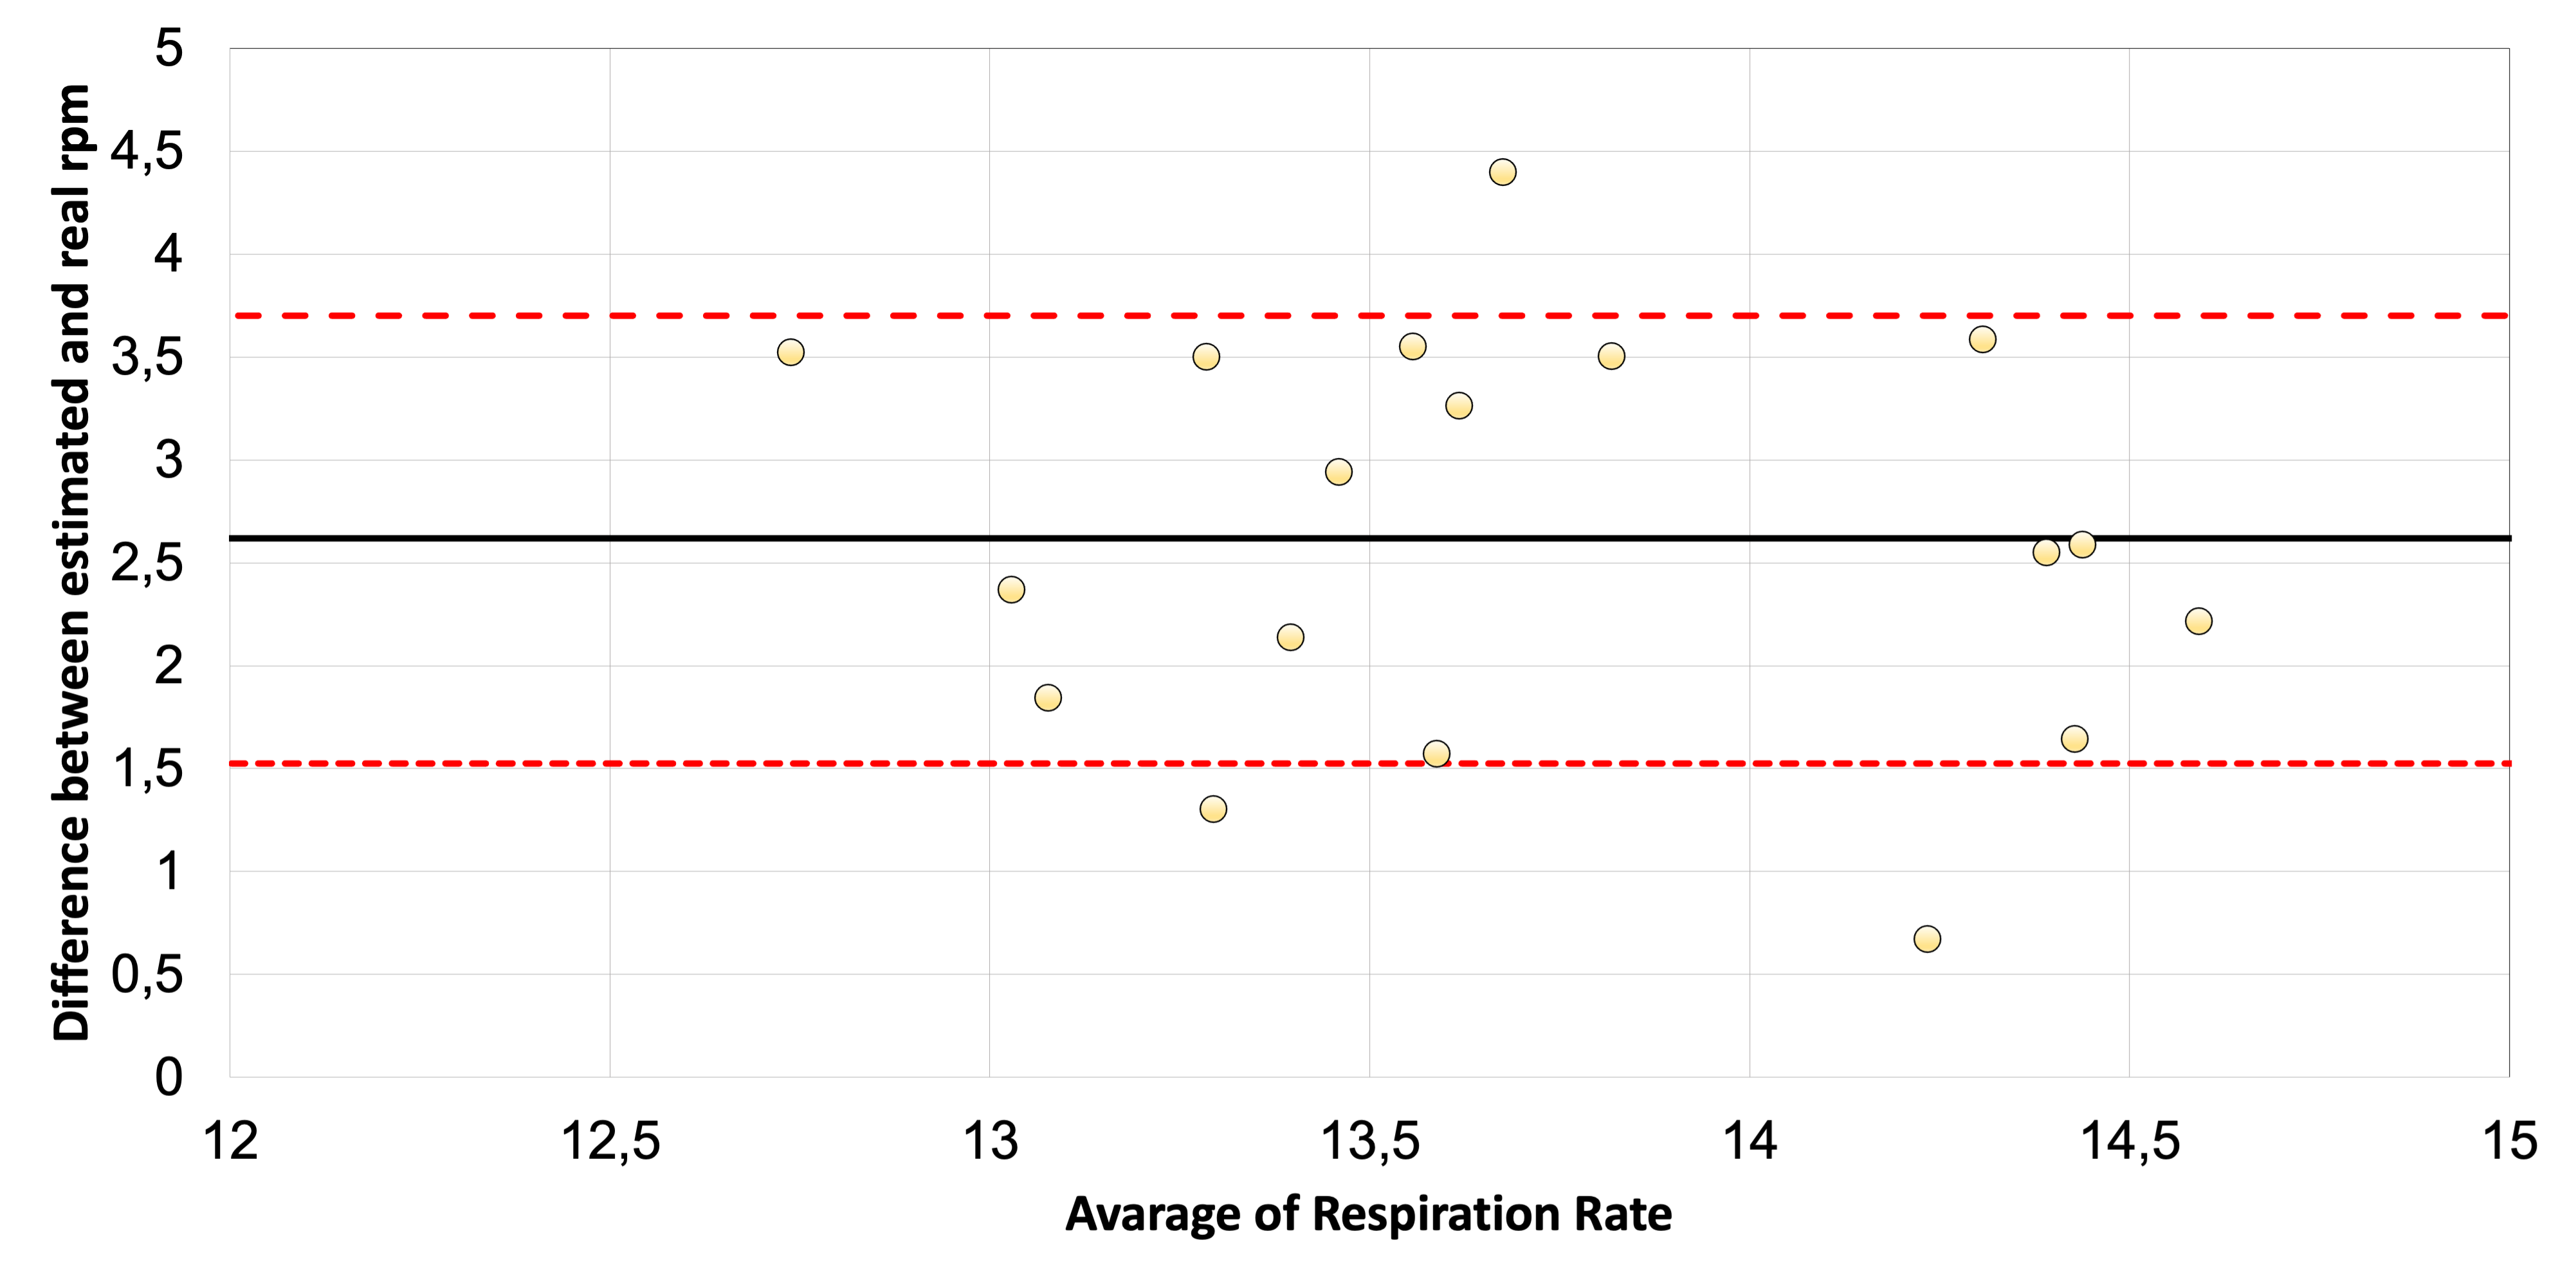
\includegraphics[width=\textwidth]{img/balnd3.png}

  \caption{Bland Altman Plot of estimated rpm from the pipeline compared to the value of the ground truth - Normal bed and prone position}
  \label{fig:baln2}
  \vspace{1.5cm}
  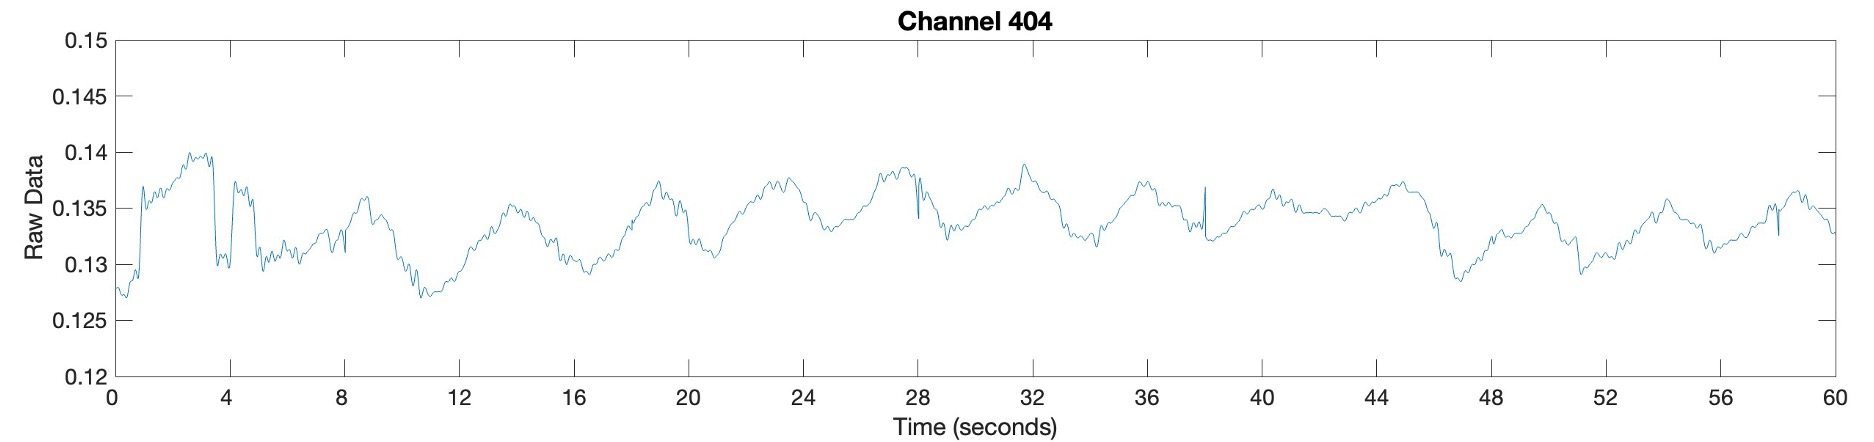
\includegraphics[width=\textwidth]{img/404.jpg}
  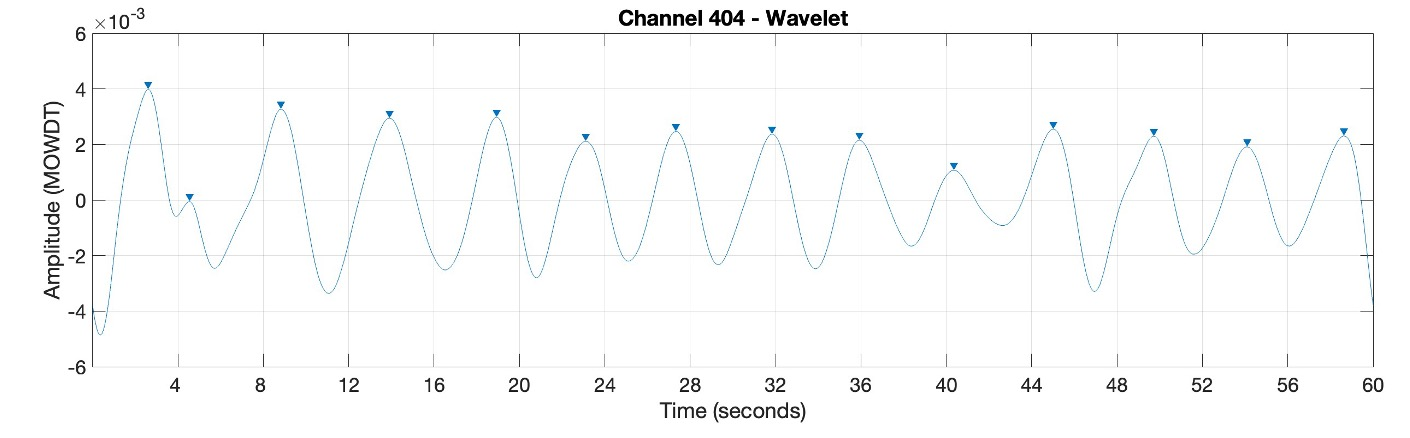
\includegraphics[width=\textwidth]{img/404_wave.jpg}
\caption{Raw data and denoised signal using MODWTMRA of the channel with the highest percentage of confidence (92\%) - Normal bed and supine position}
  \label{fig:rec}
\end{figure}

\clearpage
%%%%%% NORMAL BED - RIGHT %%%%%%
\subsubsection{Result Normal Bed in Right Side Position}   \label{cap:ResultNormalBed4}

The estimated respiratory rate per minute (rpm) while the participants are on the right side with the mattress placed on a normal bed is further presented. Table \ref{tab:RightNormalStillsg} presented the estimated rpm using binary and weighted approach compared with the rpm given by the ground truth. The approaches retrieve an almost identical rpm, this result may be due to the choice of the minimum confidence value at 80\% that allows keeping only the best signal, maybe with higher confidence can be seen a higher difference between the two approaches. 

\vspace{1cm}
%\begin{table}\begin{tabular}{|llllll|}
\hline 
Binary SGf & binary Waveleft & weighed  SGf & weighed Waveleft & resp rate & toolbox \\ 
\hline 
13.375 & 14.6364 & 13.375 & 14.6364 & 11.2045 & 10 \\ 
13.6667 & 15 & 13.6667 & 15 & 12.7397 & 11 \\ 
14 & 16 & 13.5 & 15.25 & 13.0613 & 12 \\ 
14.3571 & 14.2 & 14.3571 & 14.2 & 12.2669 & 12 \\ 
14 & 19 & 14 & 19 & 12.1628 & 13 \\ 
12.8 & 15 & 12.6667 & 14.5 & 13.6039 & 13 \\ 
11.8 & 14.2222 & 11.8 & 14.2222 & 13.1398 & 13 \\ 
14 & 15.6667 & 14 & 15.6667 & 11.5445 & 14 \\ 
13.8333 & 14.7 & 13.8333 & 14.7 & 10.77 & 11 \\ 
13.8889 & 15.8571 & 13.8889 & 15.8571 & 14.2216 & 12 \\ 
13.0833 & 15.5556 & 13.0833 & 15.5556 & 13.1656 & 12 \\ 
14.1111 & 16.5714 & 13.7 & 16.5714 & 12.9764 & 12 \\ 
14.2 & 15 & 14.2 & 15 & 10.9055 & 13 \\ 
13.25 & 15.125 & 13.25 & 15.125 & 13.2294 & 11 \\ 
12.7692 & 15.7143 & 12.2857 & 15.5 & 12.8524 & 11 \\ 
13.9167 & 15.2 & 13.6154 & 15.2 & 11.3824 & 13 \\ 
13 & 14.6 & 13 & 14.6 & 13.5579 & 11 \\ 
13 & 15.8889 & 13 & 15.8889 & 11.6069 & 12 \\ 
\hline 
\end{tabular}
\caption{Breath per minutes for each approach, result from Noxtural and toolbox
- Left position still mattress}
\end{table}

\begin{table}[h]
    \centering
    \begin{tabular}{|c|c|c|}
 
    \hline 
    Binary & Weighed & RPM (NOXA1) \\ 
    
    \hline 
    14.5714& 14.5714  & 12.4771  \\ 
    14  & 14 & 13.0835  \\ 
    16.5 & 16.5 & 14.3858  \\ 
     15.25  & 15.25 & 12.7261  \\ 
    14.5 & 14.5  & 13.4867  \\ 
    13.9333  & 13.9333  & 12.9816  \\ 
    15  & 15  & 14.0566  \\ 
    13.7692  & 13.7692  & 12.038 \\ 
    14  & 14  & 11.4923  \\ 
    14.6  & 14.6  & 11.9625  \\ 
    15  & 14.3333  & 11.0151  \\ 
    16.5  & 16.5  & 11.9016  \\ 
    14.5  & 14.5  & 11.4255  \\ 
    12.2857  & 12.2857  & 12.5227  \\ 
    12.8333  & 12.8333 & 11.5945 \\ 
    12.3333  & 12.3333  & 13.4141  \\ 
    12.3636  & 12.4783  & 13.5282  \\ 
    13.4286  & 12.875  & 12.9839  \\ 

    \hline 
\end{tabular}
\caption{Estimated rpm using binary and weighted approach of the pipeline
compared with the rpm given by the ground truth
- Normal bed and right side}
\label{tab:RighttNormalStillsg}

\end{table}

\vspace{0.5cm}

Table \ref{tab:RightNormalStillMetricssg} present the average rpm for both approaches  
and the relative mean absolute error (MAE) and mean absolute percentage error (MAPE). As just discussed in the previous paragraphs there is no substantial difference between the two different approaches. The data on which to focus more is the number of breaths that the algorithm misses, represented by MAE and expressed in percentage by MAPE. The average number is 2.5rpm, which means that if we consider the estimated average of 15rpm the error is almost 20\%, worst than in the supine position but better than in the prone position and left side.

\vspace{1cm}
\begin{table}[H]
    \centering
    \begin{tabular}{|c|c|c|}
    \hline 
    & Binary SGf & Weighed  \\ 
\hline
resp rpm & 14.523 &14.433 \\
    MAE resp & 1.8214 &     1.7593  \\ 
    MAPE resp & 14.9336 \% & 14.4066 \%\\ 


    \hline 
\end{tabular}

\caption{Evarage number of breath for each approach with the relative mean
absolute error (MAE) and mean absolute percentage error (MAE) - Normal bed
and right side}
\label{tab:RightNormalStillMetricssg}    
\end{table}
\vspace{0.5cm}

Figure \ref{fig:baln4} show the Bland–Altman plot, presented in section \ref{cap:plottino}, of the estimated rpm from the pipeline compared to the value of the ground truth. It helps to visualize the data from Table \ref{tab:RightNormalStillMetricssg} in respect of the error. Since the result for the approaches is similar the data presented with this plot refers to the weighted approach only.

Figure \ref{fig:rec4} shows the denoised signal using MODWTMRA with the highest accuracy (92\%) for the supine position with a normal mattress.

\begin{figure}[p]
  \centering
  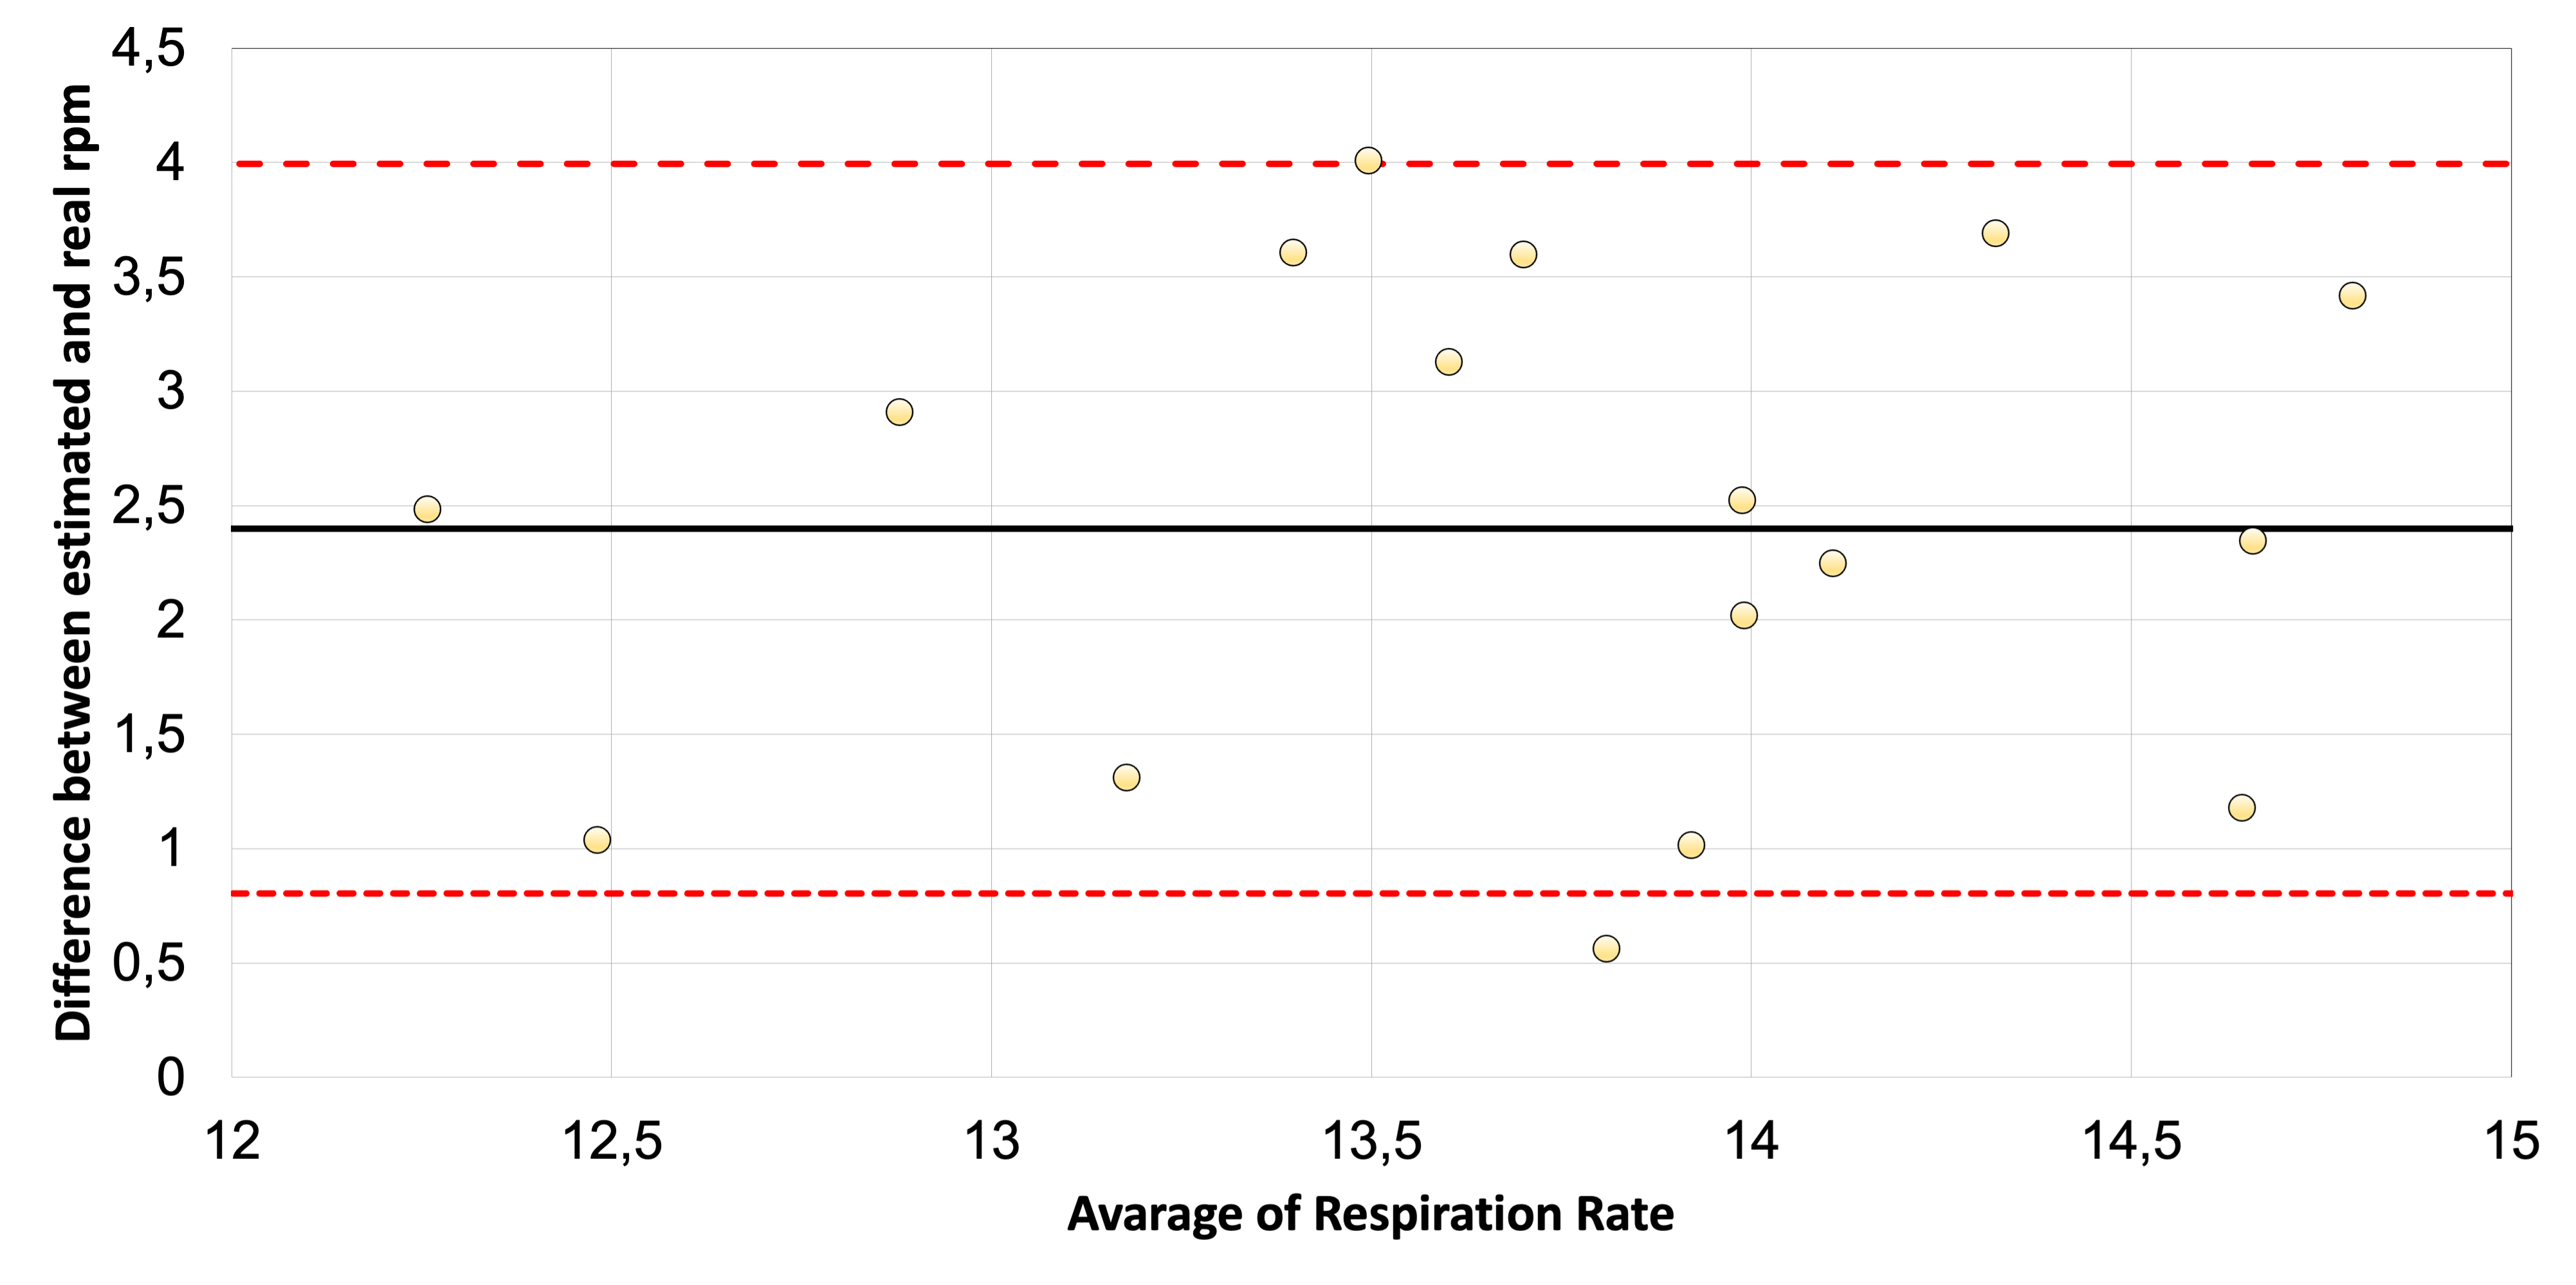
\includegraphics[width=\textwidth]{img/balnd4.png}

  \caption{Bland Altman Plot of estimated rpm from the pipeline compared to the value of the ground truth - Normal bed and left side}
  \label{fig:baln4}
  \vspace{1.5cm}
  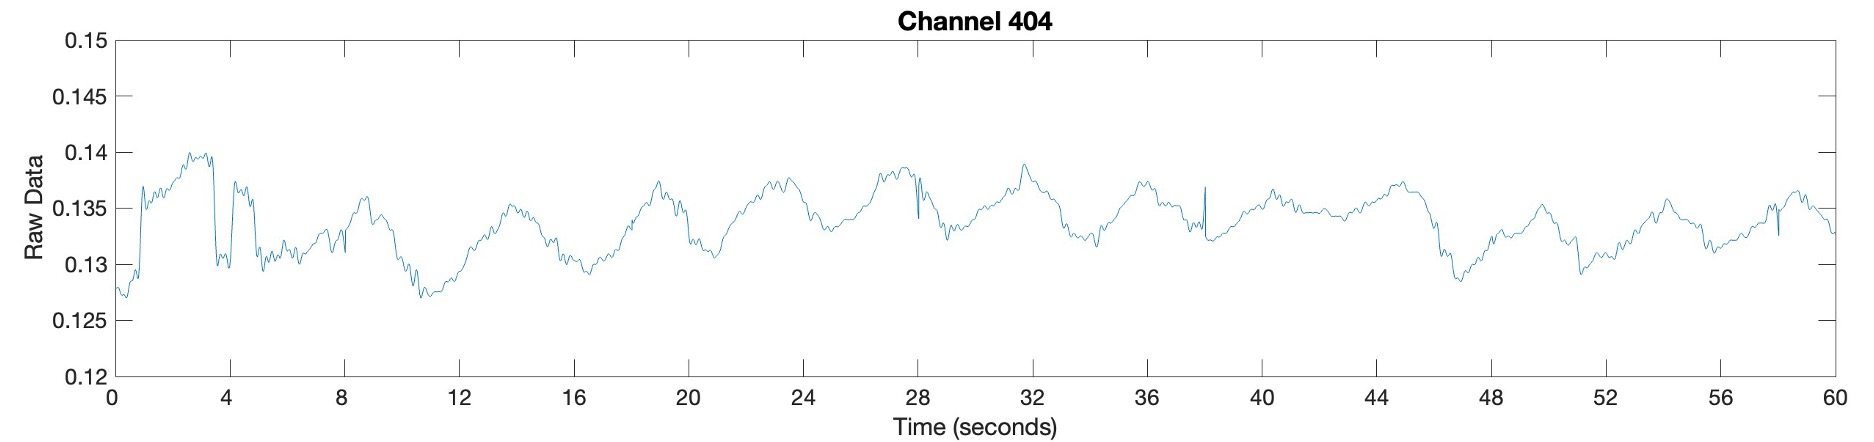
\includegraphics[width=\textwidth]{img/404.jpg}
  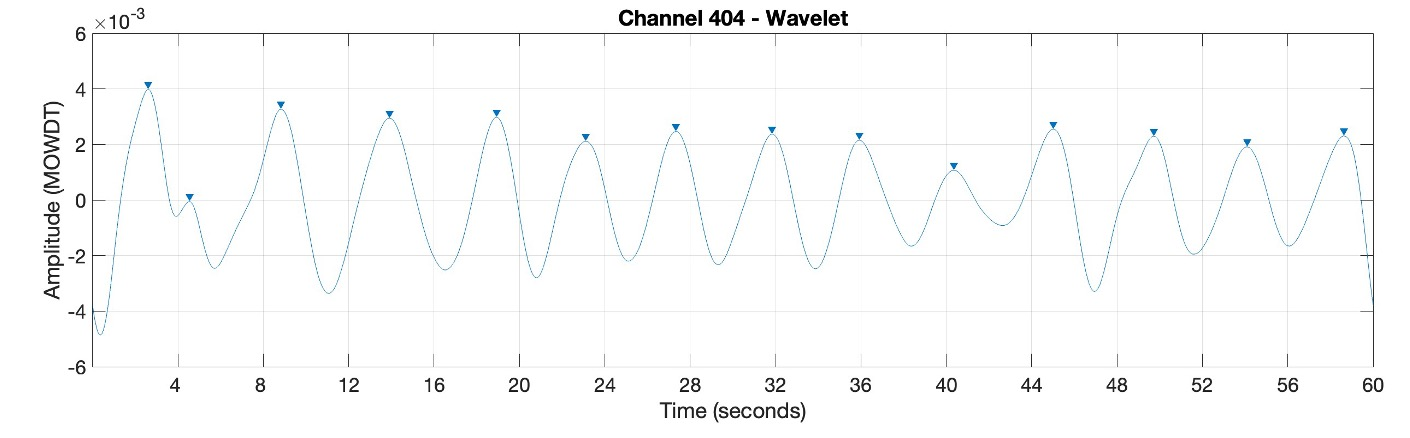
\includegraphics[width=\textwidth]{img/404_wave.jpg}
\caption{Raw data and denoised signal using MODWTMRA of the channel with the highest percentage of confidence (92\%) - Normal bed and supine position}
  \label{fig:rec4}
\end{figure}





\clearpage
%%%%%% Rocking BED - LEFT %%%%%%
\subsubsection{Result Rocking Bed in Left Side Position}  % \label{cap:ResultNormalBed1}

The estimated respiratory rate per minute (rpm) while the participants are in left side position with the mattress placed on a rocking bed is further presented. 

Table \ref{tab:LeftMovsg} presented the estimated rpm using binary and weighted approach compared with the rpm given by the ground truth. The approaches retrieve an almost identical rpm. 

\vspace{0.5cm}
\begin{table}[h]
    \centering
    \begin{tabular}{|c|c|c|}
 
    \hline 
    Binary & Weighed & RPM (NOXA1) \\ 
    \hline 
13.6875  &    13.6875   &   13.6613 \\ 
14.5294   &   14.5294    &  11.4545 \\ 
14.5     &    14.5    &  12.3288 \\ 
13.9444  &    13.9444  &    10.8865 \\ 
14.0455   &   14.0455   &   11.4082 \\ 
13.44    &  13.4231   &   12.2589 \\ 
13.9091   &   13.9091   &   13.7093 \\ 
14        &   14   &   12.7019 \\ 
14.4     &    14.4  &    13.3305 \\ 
14.5769   &   14.5769  &    13.7078 \\ 
14.7      &   14.7 &     13.5674 \\ 
14.8421   &   14.8421 &     11.8694 \\ 
14.85     &   14.85    &  13.4086 \\ 
15.5      &   15.5    &  13.9781 \\ 
13.6667  &    13.6667 &     12.4749 \\ 
13.8571   &   13.8571  &    12.4049 \\ 
13.375    &     13.7    &  13.4108 \\ 
13.75    &  14.1667      &13.4716 \\ 
\hline 
\end{tabular}
\caption{Estimated rpm using binary and weighted approach of the pipeline compared with the rpm given by the ground truth - Rocking bed and left side}
\label{tab:LeftMovsg}

\end{table}

Table \ref{tab:LeftRockingMetricssg} present the average rpm for both approaches  
and the relative mean absolute error (MAE) and mean absolute percentage error (MAPE). As just discussed in the previous paragraph there is no substantial difference between the two different approaches. The data on which to focus more is the number of breaths that the algorithm misses, represented by MAE and expressed in percentage by MAPE. The average number is 2.5rpm, which means that if we consider the estimated average of 15.2rpm the error is almost 20\%, which is too high for an approach that must be used in the medical field.

%\vspace{0.5cm}

\begin{table}[h]

    \centering

\begin{tabular}{|c|c|c|c|c|}
\hline 
& Binary & Weighed \\ 
 
\hline 
rpm mean & 13.9068 &  13.9148  \\  
MAE rpm   &   1.4229&      1.4592 \\ 
MAPE   & 11.6751\% &  11.9443\% \\ 

\hline 
\end{tabular}
\caption{Evarage number of breath for each approach with the relative mean
absolute error (MAE) and mean absolute percentage error (MAE) - Rocking bed
and left side}
\label{tab:LeftRockingMetricssg}
\end{table}

Figure \ref{fig:baln1} show the Bland–Altman plot, presented in section \ref{cap:plottino}, of the estimated rpm from the pipeline compared to the value of the ground truth. It helps to visualize the data from Table \ref{tab:LeftRockingMetricssg} in respect of the error. Since the result for the approaches is similar the data presented with this plot refers to the weighted approach only.

Figure \ref{fig:rec} shows the denoised signal using MODWTMRA with the highest accuracy (92\%) for the supine position with a normal mattress.

\begin{figure}[p]
  \centering
  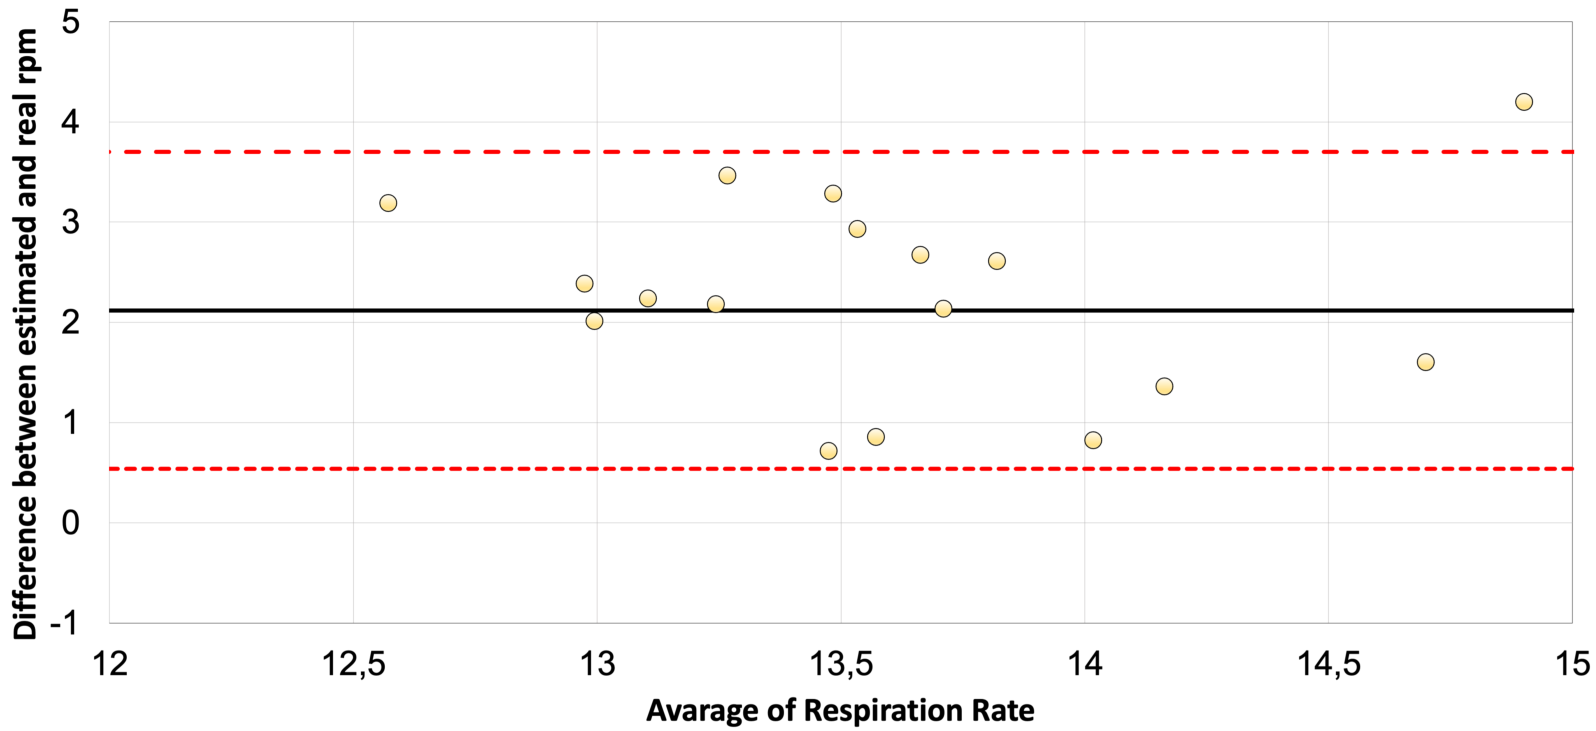
\includegraphics[width=\textwidth]{img/balnd1.pdf}

  \caption{Bland Altman Plot of estimated rpm from the pipeline compared to the value of the ground truth - Normal bed and supine position}
  \label{fig:baln1}
  \vspace{1.5cm}
  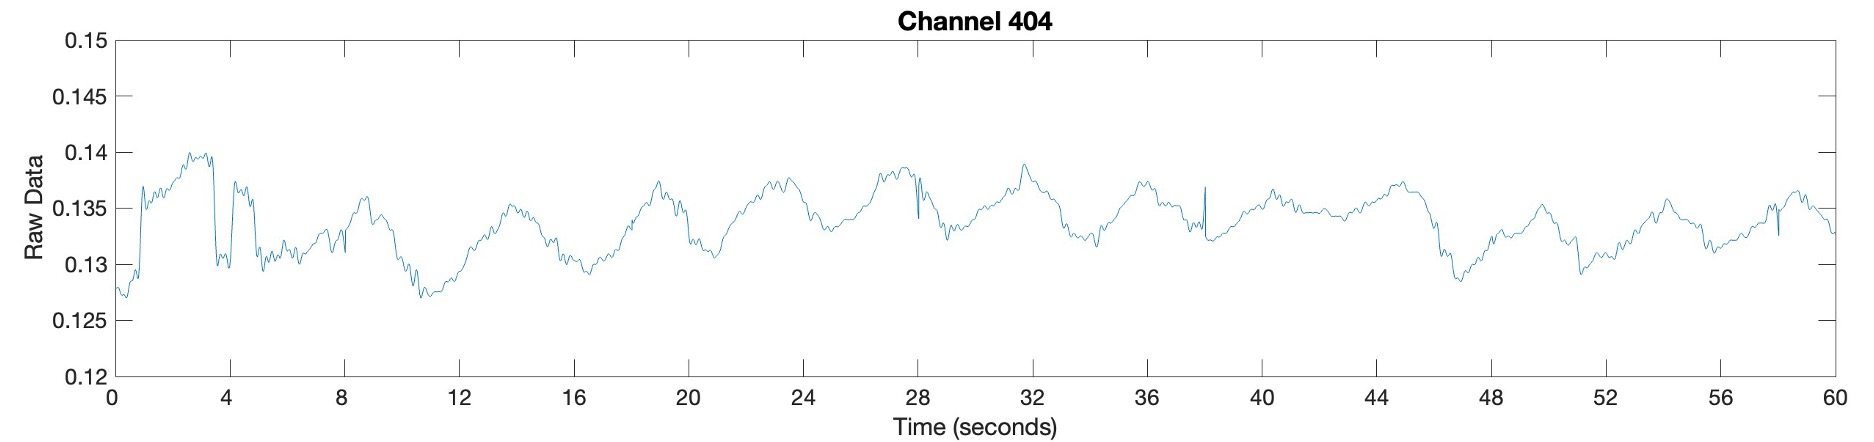
\includegraphics[width=\textwidth]{img/404.jpg}
  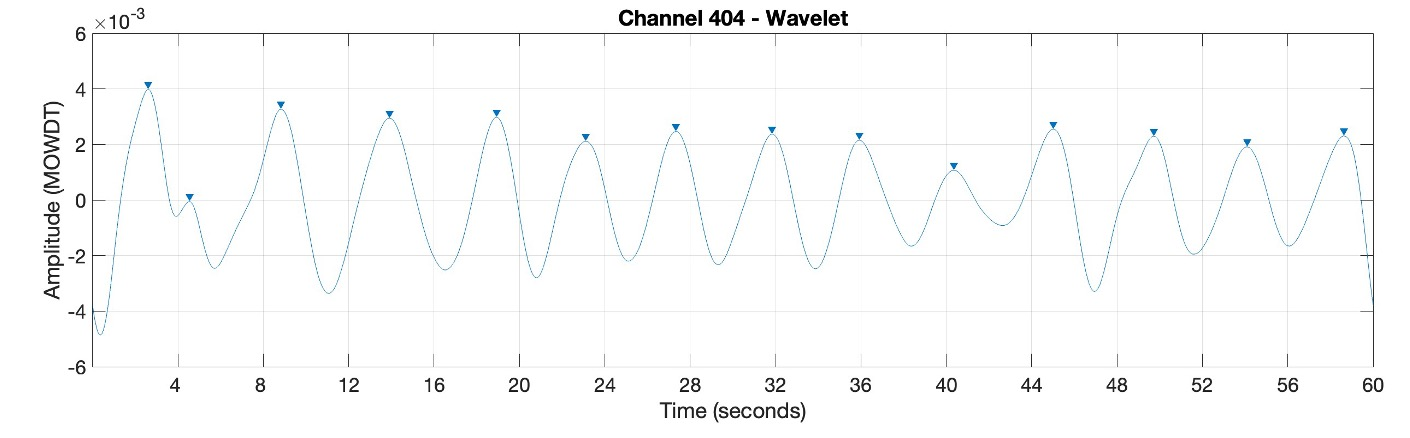
\includegraphics[width=\textwidth]{img/404_wave.jpg}
\caption{Raw data and denoised signal using MODWTMRA of the channel with the highest percentage of confidence (92\%) - Normal bed and supine position}
  \label{fig:rec}
\end{figure}

\clearpage
%%%%%% Rocking BED - Prone %%%%%%
\subsubsection{Result Rocking Bed in Prone Position}  % \label{cap:ResultNormalBed1}

The estimated respiratory rate per minute (rpm) while the participants are in prone position with the mattress placed on a rocking bed is further presented. 

Table \ref{tab:ProneRockingsg} presented the estimated rpm using binary and weighted approach compared with the rpm given by the ground truth. The approaches retrieve an almost identical rpm. 

\vspace{0.5cm}
\begin{table}[h]
    \centering
    \begin{tabular}{|c|c|c|}
 
    \hline 
    Binary & Weighed & RPM (NOXA1) \\  
\hline 
14.6667   &   14.6667  &    12.6296 \\ 
14.0455    &  14.0455  &     14.168 \\ 
14.3478    &  14.3478 &     13.2588 \\ 
14.381    &  14.3636  &    13.8107 \\ 
13.7143   &   13.7143  &    13.485 \\ 
14       &    14    &  12.6052 \\ 
16.1      &   16.1   &   11.0417 \\ 
15.7647   &   15.7647   &   12.9088 \\ 
14.7333   &   14.7333    &  13.0502 \\ 
14.6      &   14.6  &    11.1723 \\ 
14.3846   &   14.3846  &    14.6869 \\ 
13.8889    &  13.8889  &    11.3484 \\ 
13.7273   &   13.7273   &  13.0399 \\ 
13.8235   &   13.8235  &    9.54872 \\ 
13.6111   &   13.6111   &   11.7918 \\ 
13.2667   &   13.2667   &   12.8182 \\ 
12.9375   &   12.9375   &   9.53453 \\ 
13.3     &    13.3     &  9.5416 \\ 
\hline 
\end{tabular}
\caption{Estimated rpm using binary and weighted approach of the pipeline compared with the rpm given by the ground truth - Rocking bed and prone position}
\label{tab:ProneRockingsg}

\end{table}

Table \ref{tab:ProneRockingMetricssg} present the average rpm for both approaches  
and the relative mean absolute error (MAE) and mean absolute percentage error (MAPE). As just discussed in the previous paragraph there is no substantial difference between the two different approaches. The data on which to focus more is the number of breaths that the algorithm misses, represented by MAE and expressed in percentage by MAPE. The average number is 2.5rpm, which means that if we consider the estimated average of 15.2rpm the error is almost 20\%, which is too high for an approach that must be used in the medical field.

%\vspace{0.5cm}

\begin{table}[h]

    \centering

\begin{tabular}{|c|c|c|c|c|}
\hline 
& Binary & Weighed \\ 
 
\hline 
rpm mean & 14.1829  & 14.1820   \\  
MAE rpm   &   1.9835&      1.9825 \\ 
MAPE   & 17.8949\% &  17.8879\% \\ 

\hline 
\end{tabular}
\caption{Evarage number of breath for each approach with the relative mean
absolute error (MAE) and mean absolute percentage error (MAE) - Rocking bed
and prone position}
\label{tab:ProneRockingMetricssg}
\end{table}

Figure \ref{fig:baln1} show the Bland–Altman plot, presented in section \ref{cap:plottino}, of the estimated rpm from the pipeline compared to the value of the ground truth. It helps to visualize the data from Table \ref{tab:ProneRockingMetricssg} in respect of the error. Since the result for the approaches is similar the data presented with this plot refers to the weighted approach only.

Figure \ref{fig:rec} shows the denoised signal using MODWTMRA with the highest accuracy (92\%) for the supine position with a normal mattress.

\begin{figure}[p]
  \centering
  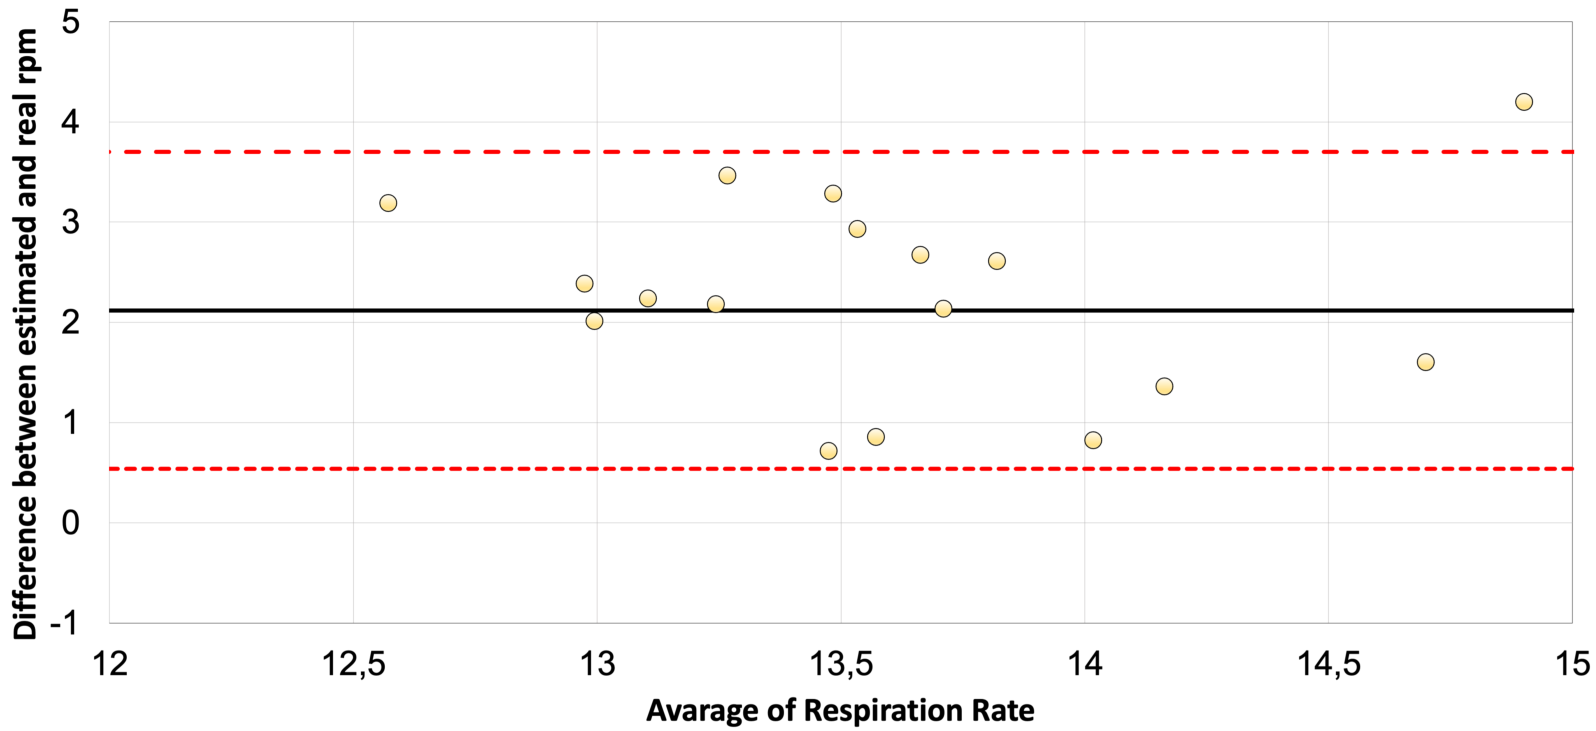
\includegraphics[width=\textwidth]{img/balnd1.pdf}

  \caption{Bland Altman Plot of estimated rpm from the pipeline compared to the value of the ground truth - Normal bed and supine position}
  \label{fig:baln1}
  \vspace{1.5cm}
  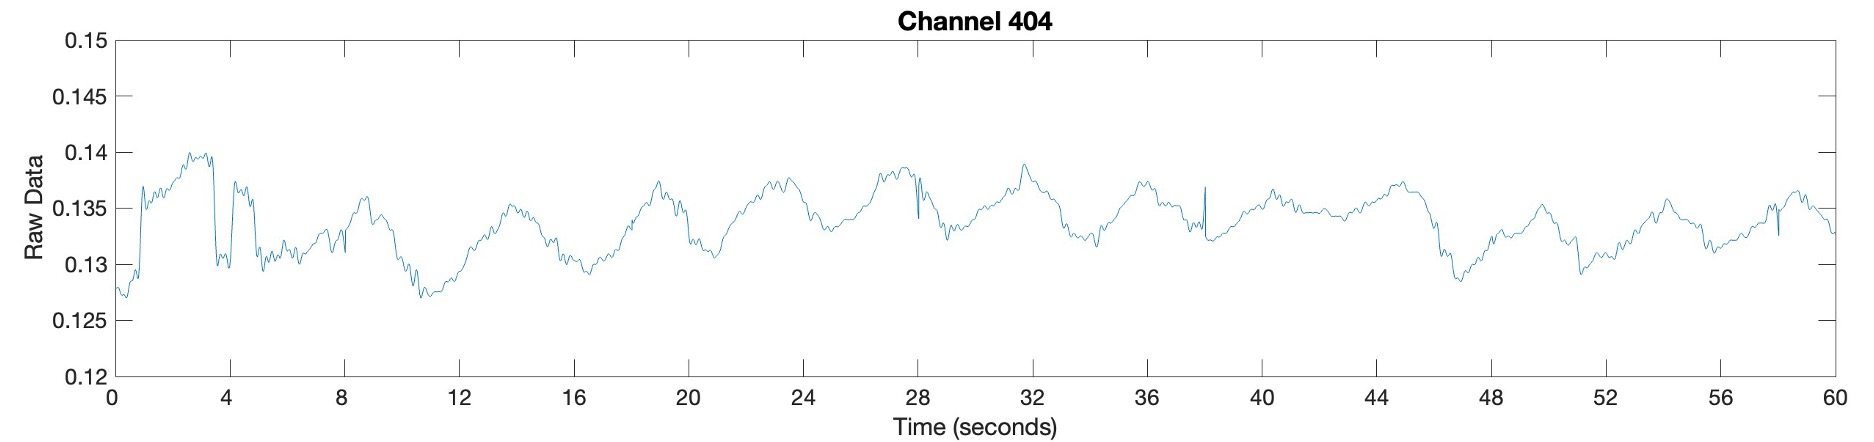
\includegraphics[width=\textwidth]{img/404.jpg}
  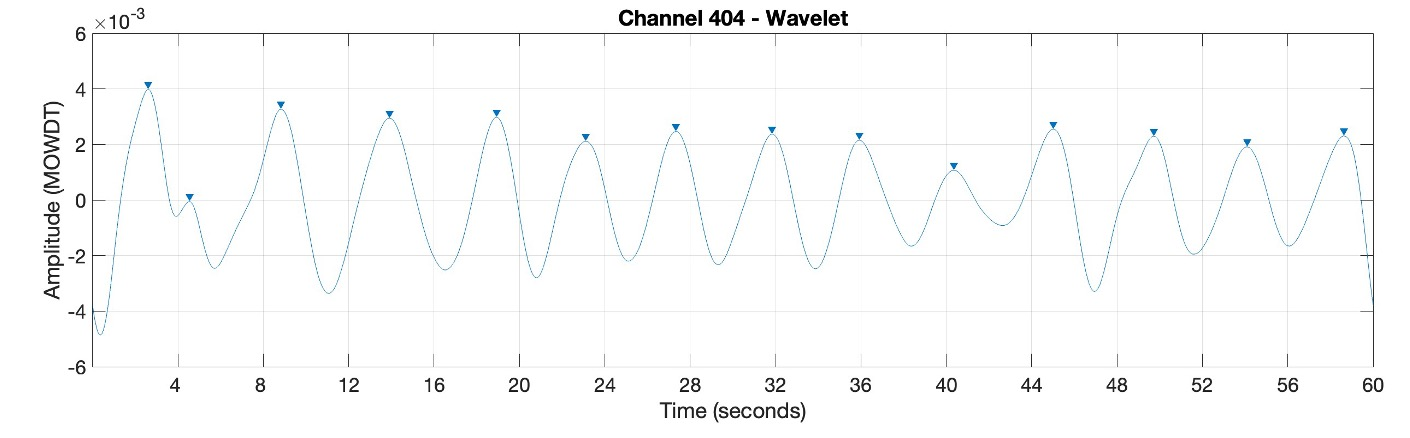
\includegraphics[width=\textwidth]{img/404_wave.jpg}
\caption{Raw data and denoised signal using MODWTMRA of the channel with the highest percentage of confidence (92\%) - Normal bed and supine position}
  \label{fig:rec}
\end{figure}


%%%%%%%%%%%%%%%%%%%%%%%%%%%%%%%%%%%%%%%%%%%%%%%%%%%%%%%%%%%%%%%%%%%%%%%%%%%%%%%%%%%%%%%%%%
\clearpage
%%%%%% Rocking BED - RIGHT %%%%%%
\subsubsection{Result Rocking Bed in Right Side }  % \label{cap:ResultNormalBed1}

The estimated respiratory rate per minute (rpm) while the participants are in right side position with the mattress placed on a rocking bed is further presented. 

Table \ref{tab:RightMovsg} presented the estimated rpm using binary and weighted approach compared with the rpm given by the ground truth. The approaches retrieve an almost identical rpm. 

\vspace{0.5cm}
\begin{table}[h]
    \centering
    \begin{tabular}{|c|c|c|}
 
    \hline 
    Binary & Weighed & RPM (NOXA1) \\  
\hline 
14.2273    &  14.2273   &   11.7955 \\ 
13.625    &  13.5294  &    11.9185 \\ 
13.9524    &  13.9524  &    11.8639 \\ 
15  &    14.7826    &    12.28 \\ 
14.5652    &   14.375  &    12.0136 \\ 
13.625    &   13.625   &   12.8838 \\ 
14.4118    &  14.4118  &    11.5695 \\ 
14.72    &    14.72  &    12.8922 \\ 
14.85    &    14.85    &   11.587 \\ 
15       &    15  &    11.2449 \\ 
15.2917   &     15.28  &    11.7082 \\ 
15.5294   &      15.5   &   13.9497 \\ 
14.5625   &   14.5294  &    11.6145 \\ 
14.8182   &   14.8182   &   13.9913 \\ 
14.7333   &   14.7333  &    11.6172 \\ 
14.8824   &   14.8824  &    13.3257 \\ 
14.75     &   14.75   &   13.5179 \\ 
15.0667   &   15.0667  &    13.5767 \\ 
\hline 
\end{tabular}
\caption{Estimated rpm using binary and weighted approach of the pipeline
compared with the rpm given by the ground truth
- Rocking bed and right side}
\label{tab:RightMovsg}

\end{table}

Table \ref{tab:RightRockingMetricssg} present the average rpm for both approaches  
and the relative mean absolute error (MAE) and mean absolute percentage error (MAPE). As just discussed in the previous paragraph there is no substantial difference between the two different approaches. The data on which to focus more is the number of breaths that the algorithm misses, represented by MAE and expressed in percentage by MAPE. The average number is 2.9rpm, which means that if we consider the estimated average of 15.3rpm the error is almost 24\%, which is too high for an approach that must be used in the medical field.

%\vspace{0.5cm}

\begin{table}[h]

    \centering

\begin{tabular}{|c|c|c|c|c|}
\hline 
& Binary & Weighed \\ 
 
\hline 
rpm mean & 14.6450  & 14.6130    \\  
MAE rpm   &   2.2367&     2.2046\\ 
MAPE   & 18.5442\% &  18.2803\% \\ 

\hline 
\end{tabular}
\caption{Evarage number of breath for each approach with the relative mean
absolute error (MAE) and mean absolute percentage error (MAE) - Rocking bed
and right side}
\label{tab:RightRockingMetricssg}
\end{table}

Figure \ref{fig:baln1} show the Bland–Altman plot, presented in section \ref{cap:plottino}, of the estimated rpm from the pipeline compared to the value of the ground truth. It helps to visualize the data from Table \ref{tab:RightRockingMetricssg} in respect of the error. Since the result for the approaches is similar the data presented with this plot refers to the weighted approach only.

Figure \ref{fig:rec} shows the denoised signal using MODWTMRA with the highest accuracy (92\%) for the supine position with a normal mattress.

\begin{figure}[p]
  \centering
  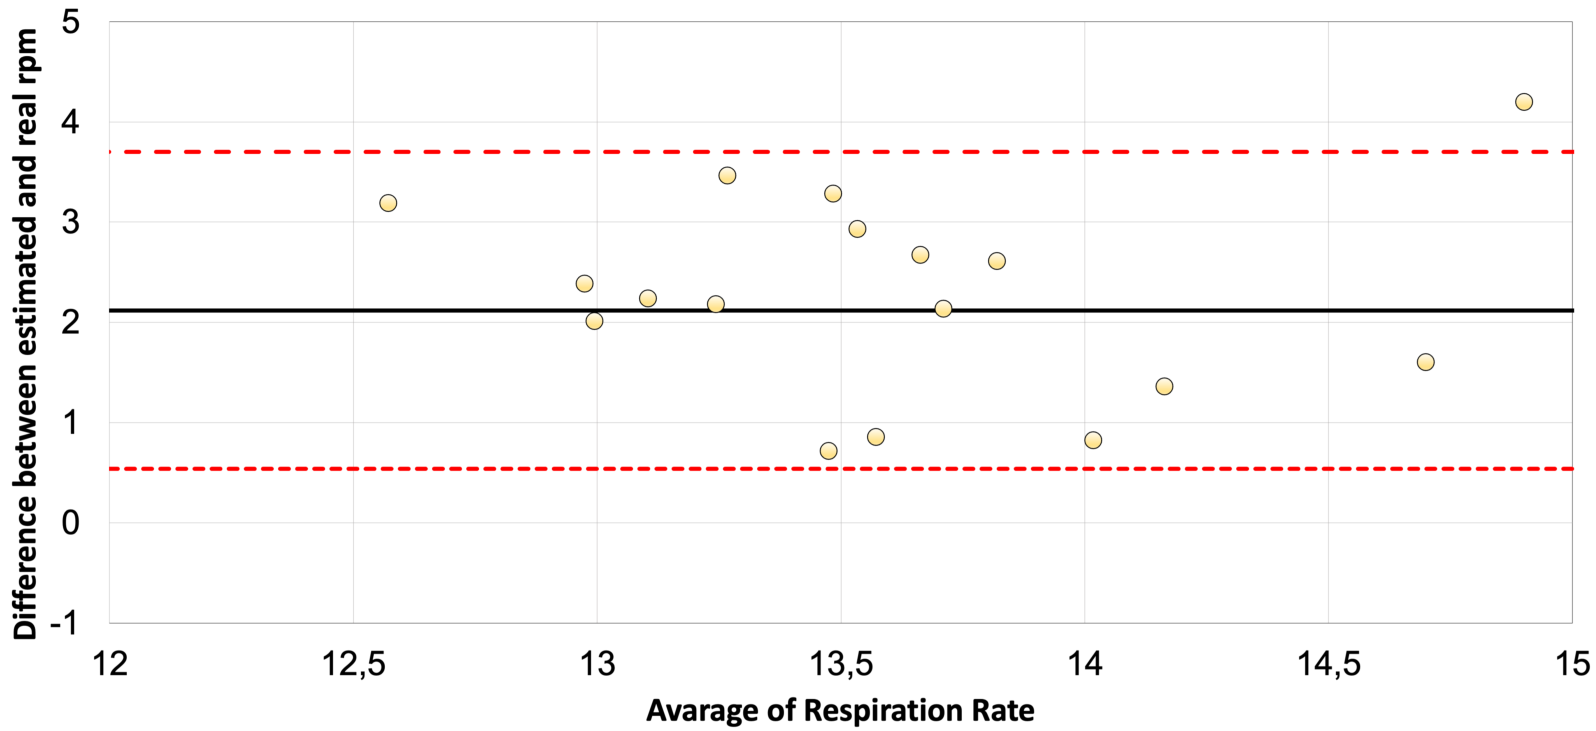
\includegraphics[width=\textwidth]{img/balnd1.pdf}

  \caption{Bland Altman Plot of estimated rpm from the pipeline compared to the value of the ground truth - Normal bed and supine position}
  \label{fig:baln1}
  \vspace{1.5cm}
  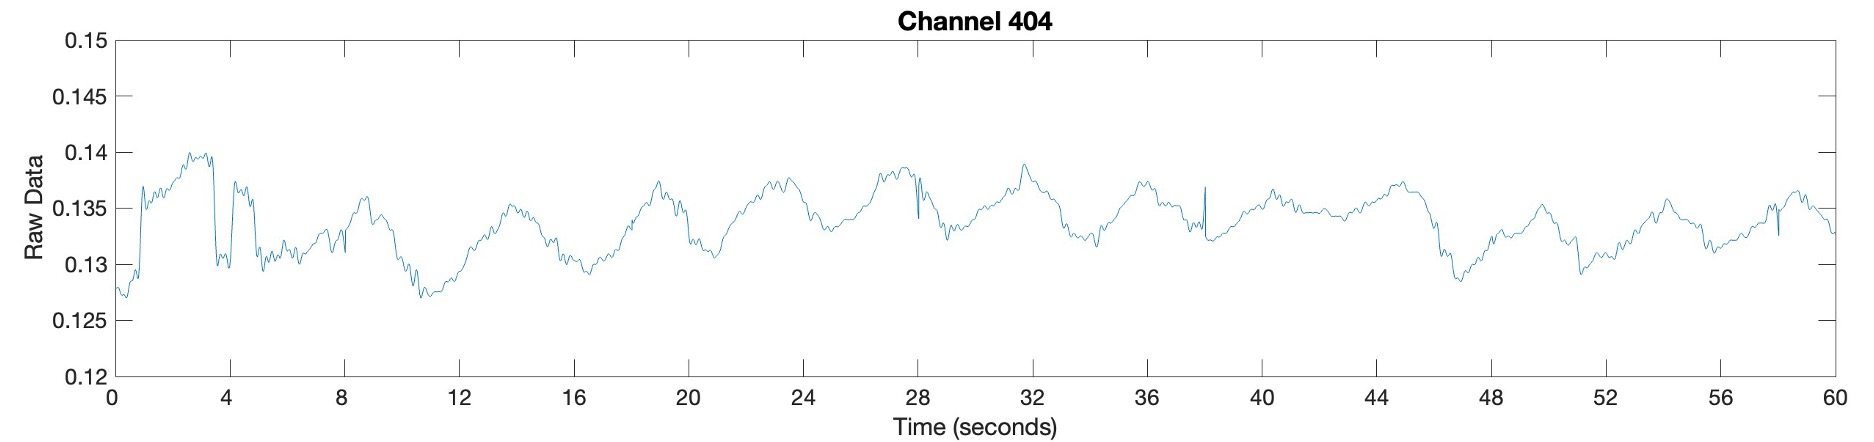
\includegraphics[width=\textwidth]{img/404.jpg}
  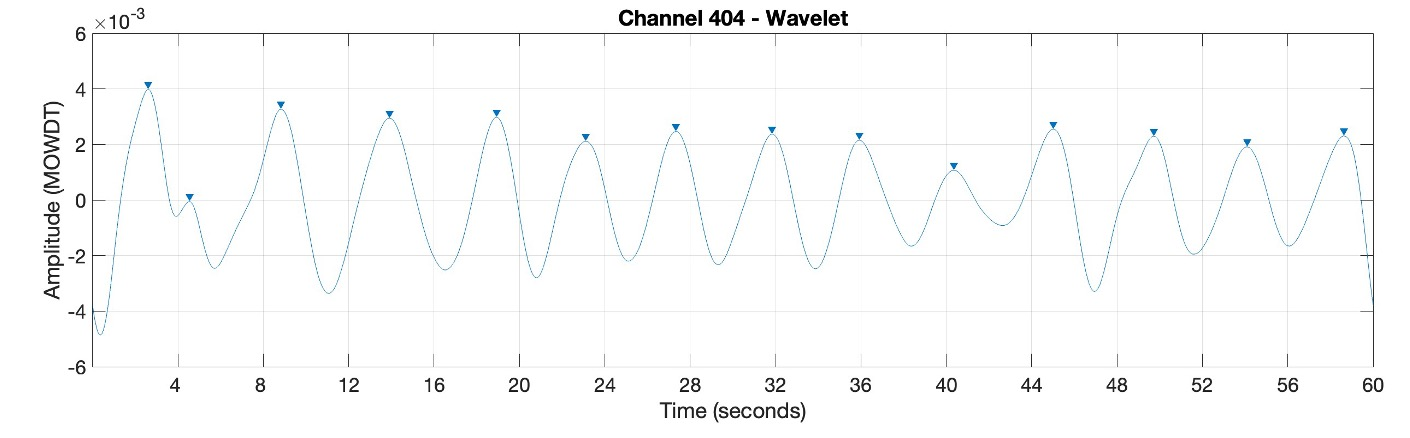
\includegraphics[width=\textwidth]{img/404_wave.jpg}
\caption{Raw data and denoised signal using MODWTMRA of the channel with the highest percentage of confidence (92\%) - Normal bed and supine position}
  \label{fig:rec}
\end{figure}